\documentclass[12pt,a4paper]{article}
\usepackage{graphicx}
\usepackage{cite}
\usepackage{latexsym}
\usepackage{fullpage}
\usepackage{gensymb}

\title{Comparing the Performance of Modified OLSR Protocols}
\author{Callan Gray, Nathan Stanley, James Udiljak}
\date{\today}

\begin{document}

\maketitle

\begin{abstract}
We compare the performance of the standard optimized link state routing (OLSR) protocol for ad-hoc wireless networking with several modified versions. The first modification involves including all one-hop neighbours of a node in that node's MPR set. Secondly, we modify OLSR to choose a random subset of the regular MPR set for each node, which is half the size of the original MPR set. Thirdly, we modify topology control (TC) messages sent by nodes to contain a random, half-length subset of the original MPR set. Finally we remove the condition that links to nodes in a node's MPR set must be bidirectional. Using ns-3, we compare the performance of these modified OLSR protocols to each other, as well as the original, unmodified protocol, for a network of 50 mobile nodes in a 1.5km by 1.5km area, each transmitting constant bit rate (CBR) traffic.
\end{abstract}

\section{The OLSR protocol}
Optimized link state routing (OLSR) is a networking protocol of the link state class. OLSR was designed to service the transmission of data across wireless networks of mobile nodes, without the use of a central router\cite{clausen2003optimized}. The first routing algorithm utilising link state routing was published in 1978 \cite{mcquillan1978arpanet}. It was developed for use in ARPANet. OLSR is based on traditional link state algorithms, but is optimised for wireless, ad-hoc networks. In link state routing protocols, every node constructs its own map of the network, represented by a graph. Nodes use this graph to independently calculate routing tables, which detail the node's best known path to each other node in the network. Only information about network topology is shared between nodes. By comparison, in distance vector routing protocols, routing tables, or parts thereof, are shared between nodes.

\subsection{The MPR Set}
Each node maintains a set of nodes which it considers multipoint relays (MPRs), termed that node's MPR set. The nodes in an MPR set are the nodes which are selected by that node to forward its broadcast messages. Packets containing information about network topology (termed topology control, or TC messages) are then only generated by nodes which have been elected as an MPR by some other node. By generating MPR sets that allow a node to broadcast to and receive from the entire network with minimal redundancy, OLSR reduces its overhead of TC messages.

\subsection{Modification 1}
The first modification to the OLSR algorithm that we test involves modifying the generation of MPR sets such that all one-hop neighbours of a node will appear in that node's MPR set, as opposed to the minimum subset of those required to allow that node to reach the entire network. We expect that this will increase the overhead of TC messages throughout the network and thus reduce throughput of data. 

The ``olsr-routing-protocol.cc" file contains a method ``MprComputation" where the MPR set is computed for each node. The base implementation of this method starts the final MPR set calculation by checking the condition that a neighbor's ``willingness" attribute is set to ``OLSR\_WILL\_ALWAYS" (this means that the neighbour will always be willing to forward packets from that node). To implement modification 1, we override this, adding all neighbors to the MPR set. 

\subsection{Modification 2}
We also modify OLSR to choose a random subset of the traditionally generated MPR set for each node, which will be used as its MPR set. Since the MPR sets are usually generated to be as small as possible without reducing the node's ability to reach other nodes in the network, we expect that this will make some links unserviceable, causing throughput to drop.

As above, the changes are made in the ``MprComputation" method, which calculates the MPR set for each node. At the end of this method, prior to being set on the ``m\_state" variable, the MPR set is converted to a list, which is then randomised and the first \(n\) elements selected as the modified MPR set, where \(2n\) is the initial size of the MPR set. As the list has been shuffled, simply taking the top half, rounded up for an odd number of neighbors, is sufficient to ensure a fairly chosen random subset.

\subsection{Modification 3}
By modifying TC messages so that nodes only send half of their MPR set to other nodes, nodes will be rendered unaware of the existence of some nodes within the network. We expect that this will again render some links in the network unserviceable, again causing throughput to drop.

The file ``olsr-routing-protocol.cc" contains a method ``SendTc" which gets the MPR selector set and sends the full set as part of a toplogy control message. Our implementation of modification 2 is similar to that or modification 2: The set is converted to a list, randomised, the top half is skimmed, and the subset is sent in place of the full MPR selector set.

\subsection{Modification 4}
Finally, we modify OLSR, by removing the condition that a bidirectional link exist between a node and all its neighbors in the MPR set. In the standard OLSR algorithm, for a node \(A\) to be in node \(B\)'s MPR set, node \(B\) must be in node \(A\)'s MPR set. We expect this to reduce the throughput of the network as some links which are expected to exist by a given node, will not.

To implement modification 4, we note that the method ``LinkTupleUpdated" is called when a link tuple is changed. In this method, the bi-directional link condition is checked. By overriding the bi-directional link flag to True, the check is bypassed, allowing unidirectional links to exist.

\section{ns-3}
ns-3 is an open source network simulation framework with an extensive array of plugins. ns-3 is capable of simulating every layer of networking from physical to application. It allows for the simulation of mobile nodes communicating wirelessly through an ad-hoc network. We use ns-3 to test the performance of the standard OLSR protocol, and each of our four modifications. We use a 50 node network, with nodes confined in a \(1500\) by \(1500m\) space, moving at \(1\), \(10\), and \(20ms^{-1}\). We test the network with \(10\), \(20\), and \(30\) nodes generating constant bitrate traffic, analysing network throughput.

\pagebreak
\section{Results}

\begin{figure}[ht]
\centering
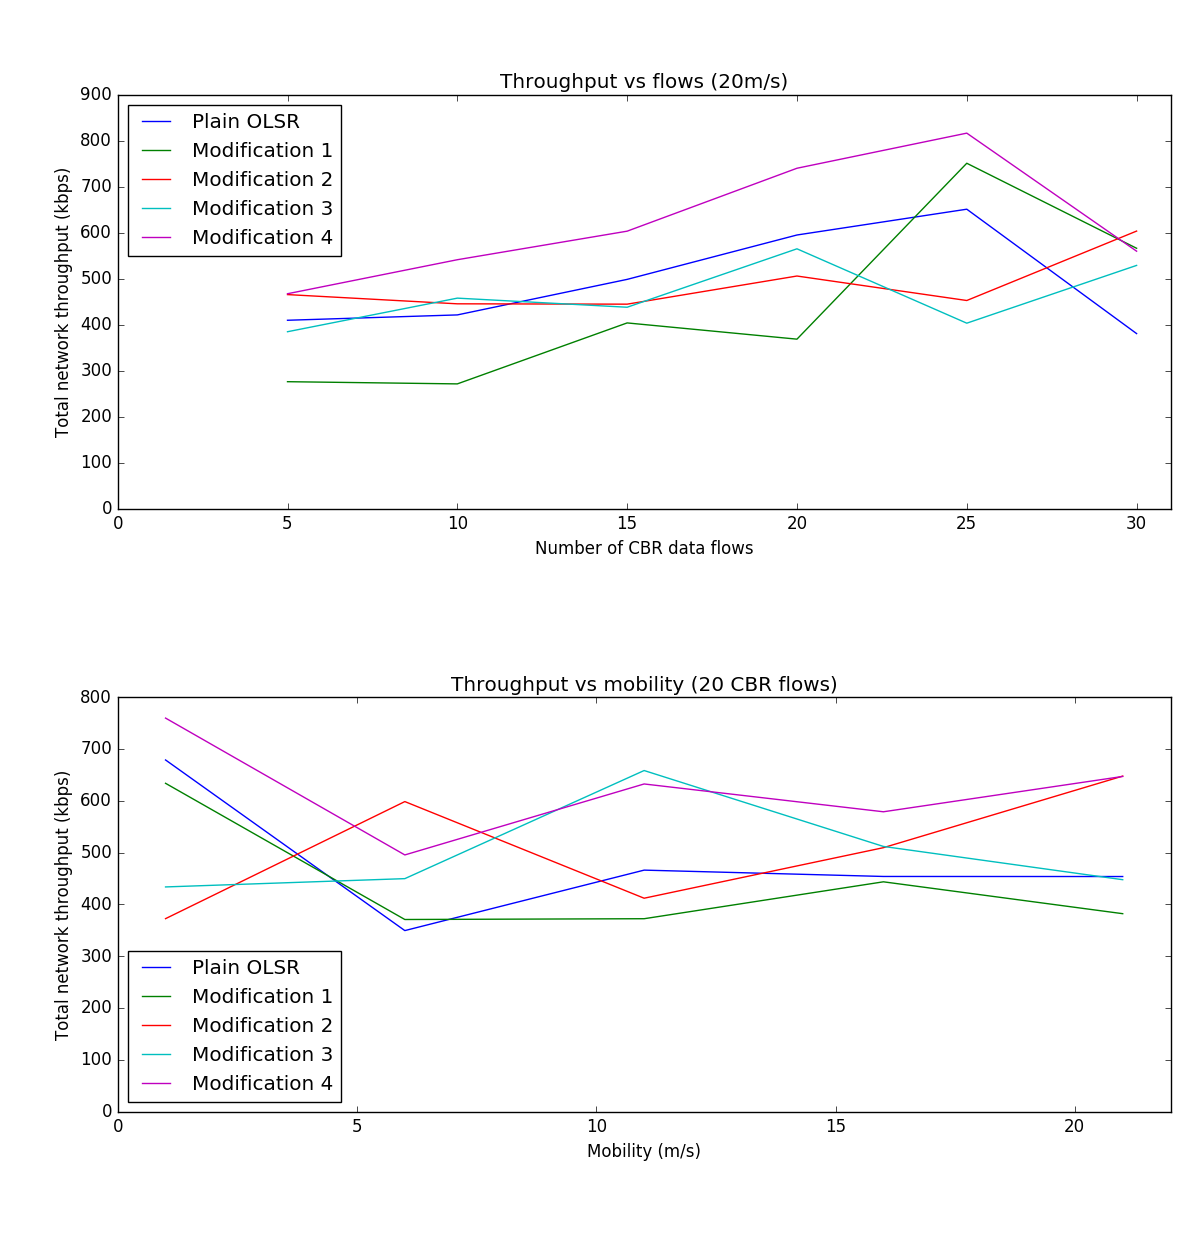
\includegraphics[width=\textwidth]{figure_1}
\end{figure}

\section{Conclusion}
Modification 1, shown as the green plot, performed worse than plain OLSR for all but the two highest data flow rates tested. This is as we expected. Including all the neighbours in the MPR set increases congestion throughout the network for broadcast traffic. In this case, the broadcast traffic across our network is limited to OLSR's own messages. By increasing OLSR's traffic, we decrease the throughput available to the application layer.

Modification 2, the red plot, also performed significantly worse than plain OLSR. This is again as we predicted. By removing half of each node's MPR set, we see some links become unserviceable, and thus throughput is lowered. The performance of modification 2 shoots up above that of plain OLSR in the 30 data flow case. We posit that this is because in a situation where there are more data sources than sinks, some sink nodes must accept data from more than one source. Modification 2 makes some links unserviceable, quite possibly meaning that these nodes now only have to receive data from one source, easing network congestion and improving throughput for the remaining link.

Modification 4, the purple plot, actually saw an increase in throughput across the board over plain OLSR. This is contrary to our expectations. We think this may be due to the fact that if there are \(n\) bi-directional paths to a node, then there are \(m \geq n\) uni-directional paths to that node. In our case, we only have uni-directional data flows, so these extra uni-directional links can be utilised to improve overall throughput.

\bibliographystyle{plain}
\bibliography{references}

\end{document}